\documentclass{l4proj}
\usepackage{tikz}
\usepackage{etoolbox}
\usepackage{listings-rust}

\usetikzlibrary{calc,arrows}

\begin{document}
\makeatletter
% make numeric styles use name format
\patchcmd{\NAT@test}{\else \NAT@nm}{\else \NAT@nmfmt{\NAT@nm}}{}{}

% define \citepos just like \citet
\DeclareRobustCommand\citepos
{\begingroup
    \let\NAT@nmfmt\NAT@posfmt
    \NAT@swafalse\let\NAT@ctype\z@\NAT@partrue
    \@ifstar{\NAT@fulltrue\NAT@citetp}{\NAT@fullfalse\NAT@citetp}}

\let\NAT@orig@nmfmt\NAT@nmfmt
\def\NAT@posfmt#1{
    \StrRemoveBraces{#1}[\NAT@temp]
    \IfEndWith{\NAT@temp}{s}
    {\NAT@orig@nmfmt{#1'}}
    {\NAT@orig@nmfmt{#1's}}}

\makeatother

\title{MQuicTT: evolving IoT at the transport layer}
\author{Ivan Nikitin}
\date{\today}

\maketitle

\begin{abstract}
    New advances in networked systems and programming languages are set to succeed existing industry standards.
    In the transport layer space, QUIC - a is set to succeed the TCP/TLS stack and is advantageous for performance and security by leveraging improved features such as a simpler, secure handshake, and streams.
    While in the programming languages space, Rust, a new systems programming language, uses a strong type system to guarantee memory-safety and deadlock-freedom, while still being performant.
    In this work we analyse the feasibility of using a Rust based QUIC implementation as the basis for secure communication in IoT devices.
    To do so, in this work we develop $MQuicTT$ - a Rust based MQTT implementation using QUIC at the transport layer.
    We compare the performance of the resulting solution with existing MQTT implementations in various use cases and analyse the hardware resources needed to deploy it.
    We find that the performance of the implementation is on par with the baseline.
    Finally, we discuss the binary size of the implementation and the possible methods to generally reduce Rust binary sizes for IoT network firmware using QUIC.
\end{abstract}

\def\consentname {Ivan Nikitin} % your full name
\def\consentdate {25 March 2022} % the date you agree
\educationalconsent


\tableofcontents

\chapter{Introduction}

% reset page numbering. Don't remove this!
\pagenumbering{arabic} 

The Internet of Things (IoT) is rapidly becoming the most prominent form of computation, with the number of IoT devices projected to surpass 75 billion by 2025~\citep{statista_number_2016}.
IoT devices range from daily consumer gadgets such as wearables to sensors that are used in smart factories.
The central theme of these devices is network connectivity.
Network firmware installed on these devices has to be performant enough to send and receive massive amounts of data. 
Hence, the need for efficient, lightweight network firmware often means that manufacturers of these devices forego security for performance~\cite{ling_iot_2018}.
Therefore, the mass use of devices that are manufactured without security in mind creates a situation where many devices that are critical to infrastructure become vulnerable to cyber attacks, as seen in the 2015 attack on the Ukraine power grid~\citep{Liang2017}.
However, we can not just employ the usual methods to secure firmware on these devices due to the presented constraints in terms of their physical size, power consumption needs and available hardware.
Hence, there is a need to develop methods for secure, performant communication for this device class.

MQTT~\citep{oasis_mqtt_2014} is a popular message-passing network protocol designed to be lightweight for the IoT use case.
While certain protocols have been developed to specifically act as data transfer protocols for IoT devices, MQTT remains the most widely used.
MQTT's design ensures that the protocol's implementations have a small code footprint and take up minimal network bandwidth.
Significantly, MQTT relies on a transport layer protocol to send data and ensure secure communication.
The standard in current MQTT implementations is to use the TCP/TLS stack to provide secure data transfer.
As we present in this work, this stack adds overhead, which means that the advantages of MQTT are negated if we need secure communication.
However, QUIC~\citep{iyengar_quic_2021}, a new transport layer network protocol initially designed at Google, is set to succeed TCP with a number of improvements.

QUIC boasts advantages in both secure communication and performance. 
Expanding the range of hardware constrained devices that MQTT can support would also work towards standardising messaging protocols for IoT devices.
As we will demonstrate in further sections, many of the available protocols rely on the same fundamentals, and it may not be desirable to support all of these.
Hence, we introduce MQuicTT - a QUIC port of an MQTT library in the Rust programming language, discuss the design choices made during its development, analyse its performance and discuss the challenges IoT presents for network protocols.
We further analyse the steps needed to create protocols for hardware constrained devices and present an analysis for the methodology of lowering the overhead of a QUIC stack.

\section{Dissertation Outline}

The rest of this dissertation is structured as follows:
\begin{itemize}
    \item Chapter~\ref{chap:back} provides a background on the recent developments in the transport layer network protocol space, IoT and the Rust programming language.
    \item Chapter~\ref{chap:libs} provides a rationale for the implementations of QUIC and MQTT that were chosen for MQuicTT.
    \item Chapter~\ref{chapter:quic_socket} details the implementation of $QuicSocket$ - an intermediate QUIC API that we have developed.
    \item Chapter~\ref{chap:net_sim} gives an explanation of our methodology for the analysis that follows in later chapters.
    \item Chapter~\ref{chapter:eval} details the analysis of MQuicTT and provides a discussion of results.
    \item Chapter~\ref{chap:TLS} discusses the pros and cons of TLS as a security protocol for IoT.
    \item Finally, Chapter~\ref{chap:conclusion} concludes and summarises important results.
\end{itemize}
\chapter{Background}

In this chapter we present the background of topics that are fundamental for this work.
We examine the current developments in the networks and systems programming spaces and identify how these apply to what we aim to achieve.

\section{The evolution of the transport layer}

In the following section we provide a background on transport layer protocols and recent advancements in the space applicable to the body of work conducted.
Together, the protocols described comprise most of the traffic on the Internet.
Hence, smaller use-case protocols that do exist were not seen as applicable.

First described by~\citet{cerf_protocol_1974}, the Transmission Control Protocol (TCP) has been the main protocol of the Internet suite since its initial implementation.
TCP provides a \textit{reliable} and \textit{ordered} delivery of bytes.
That is, TCP ensures that data is not lost, altered or duplicated and is delivered in the same order that it was sent.
This is achieved by assigning a sequence number to each transmitted packet and requiring an \textit{acknowledgment} (commonly referred to as ACK) from the receiving side.
If an ACK is not received, the data is re-transmitted.
On the receiving side, the sequence numbers can also be used to order packets as intended by the sender.

As TCP is a connection based protocol, connection establishment must take place before any data can be transmitted.
The receiving side (the server) must bind to and listen on a network port and the sender (the client) must initiate the connection using the process of a \textit{three-way handshake} as shown in Figure \ref{fig:tcp}.
In the first step of the handshake, the client sends a segment with a \textit{synchronise sequence number} (SYN) that indicates the start of the communication and the sequence number that the segment starts with.
The server responds with an acknowledgment - ACK, and the sequence number it will start its segment with - SYN.
Hence, this step is often referred to as the SYN-ACK.
In the third and final step, the client must acknowledge the response.
At this point, the connection on which data can be transferred is established.

\begin{figure}[ht]
    \begin{center}
        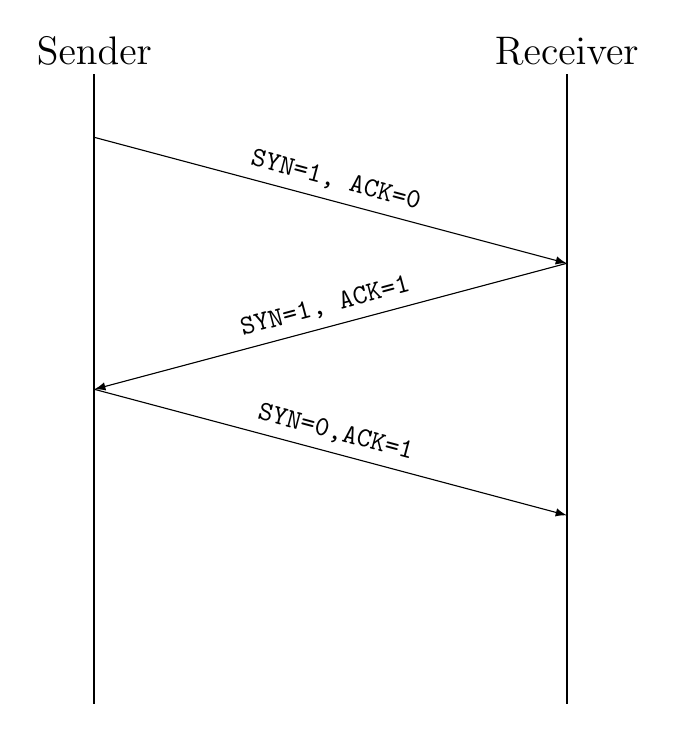
\begin{tikzpicture}[>=latex]
            \coordinate (A) at (2,8);
            \coordinate (B) at (2,0);
            \coordinate (C) at (8,8);
            \coordinate (D) at (8,0);
            \draw[thick] (A)--(B) (C)--(D);
            \draw (A) node[above]{\Large Sender};
            \draw (C) node[above]{\Large Receiver};

            \coordinate (E) at ($(A)!.1!(B)$);
            \draw (E) node[left]{\begin{tabular}{r}
                \end{tabular}};

            \coordinate (F) at ($(C)!.3!(D)$);
            \draw (F) node[right]{\begin{tabular}{l}
                \end{tabular}};
            \draw[->] (E) -- (F) node[midway,sloped,above]{\verb$SYN=1, ACK=0$};

            \coordinate (G) at ($(A)!.5!(B)$);
            \draw (G) node[left]{};
            \draw[->] (F) -- (G) node[midway,sloped,above]{\verb$SYN=1, ACK=1$};

            \coordinate (H) at ($(A)!.5!(B)$);
            \draw (H) node[right]{};

            \coordinate (I) at ($(C)!.7!(D)$);
            \draw (I) node[left]{};
            \draw[->] (H) -- (I) node[midway,sloped,above]{\verb$SYN=0,ACK=1$};
        \end{tikzpicture}
        \caption{The TCP handshake needed for connection establishment. The values of the SYN and ACK fields being set indicate the kind of segment sent. For example, for the SYN-ACK stage both the SYN and ACK fields are set.}
        \label{fig:tcp}
    \end{center}
\end{figure}

In order to achieve \textit{secure communication}, TLS~\citep{rescorla_transport_2018} is often used in the TCP stack.
In order to do this a separate TLS handshake has to occur in order to specify the version of TLS to use, decide on the cipher suites, authenticate the server via its public key and certificate authority's signature, and generate a session key that can be used for symmetric encryption during communication.
In the TLS handshake the first step is for the client to send a $ClientHello$ message that specifies the highest version of TLS that the client supports, a list of suggested cipher suites, compression methods and a random number.
The server responds with a $ServerHello$ message that contains the selected TLS version, cipher suite, compression method and its own random number.
The server then sends its certificate and $ServerKeyExchange$ message along with the $ServerHelloDone$ message indicating that it has completed its part of the negotiation process.
The client will respond with the $ClientKeyExchange$ message (CKE) which, depending on the chosen cipher suite, may contain a public key.
This is followed by the client sending a $ChangeCipherSpec$ message indicating that all communication from this point is authenticated and encrypted along with a finished message.
The server responds with the same message and the TLS connection is established.

Due to the establishment of communication and properties guaranteed by TCP, such as reliability through retransmission, an inherent trade-off is created, and latency is lengthened.
Hence, in use-cases where reliability and connection state is not required, the User Datagram Protocol (UDP)~\citep{j_postel_1980} is preferred.
UDP uses a connectionless communication model that aims to have a minimal number of semantics. The only mechanisms provided by UDP are port numbers and checksums in order to ensure data integrity.
This is preferable for real-time systems as using TCP for these would cause an overhead to latency and retransmission of packets that are no longer needed by the application.

QUIC is a relatively new general-purpose transport layer protocol originally designed by~\citet{jim_roskind_2012} at Google as part of the Chromium web engine.
In 2015 the first draft of the QUIC protocol was submitted to the IETF and was later standardised~\citep{iyengar_quic_2021}.

The aim of QUIC is to improve upon, and eventually make obsolete, TCP by using the concept of multiplexing, which is a method of combining several signals or channels of communication over one shared medium.
QUIC establishes multiplexed connections between the communicating endpoints using UDP.



QUIC facilitates data exchange on the UDP connection through the concept of \textit{streams}.
Streams are an ordered byte-stream abstraction used by the application to send data of any length.
Streams are created by either the sending or receiving side and can be both unidirectional and bidirectional.
Each side can send data concurrently on the stream and can open any number of streams (specifically, a field for the maximum number of streams is set during the connection).
Hence, subject to the constraints imposed by flow control, QUIC allows an arbitrary number of streams to send arbitrary amounts of data on the UDP connection.

By doing so, QUIC also achieves secondary goal of lifting congestion control algorithms from the kernel space to the user space.
Hence, congestion control algorithms can evolve without having to be tied down to kernel level semantics and constraints.

\begin{figure}[ht]
    \begin{center}
        \begin{subfigure}[b]{0.45\textwidth}
            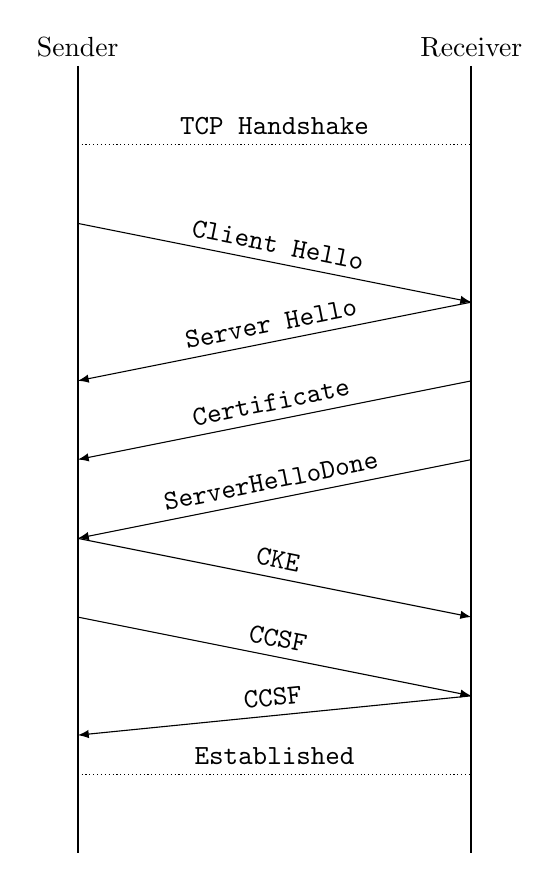
\begin{tikzpicture}[>=latex]
                \coordinate (A) at (2,10);
                \coordinate (B) at (2,0);
                \coordinate (C) at (7,10);
                \coordinate (D) at (7,0);
                \draw[thick] (A)--(B) (C)--(D);
                \draw (A) node[above]{Sender};
                \draw (C) node[above]{Receiver};

                \coordinate (H) at ($(A)!.1!(B)$);
                \draw (H) node[right]{};

                \coordinate (I) at ($(C)!.1!(D)$);
                \draw (I) node[left]{};
                \draw[densely dotted] (H) -- (I) node[midway,sloped,above]{\verb$TCP Handshake$};

                \coordinate (H) at ($(A)!.2!(B)$);
                \draw (H) node[right]{};

                \coordinate (I) at ($(C)!.3!(D)$);
                \draw (I) node[left]{};
                \draw[->] (H) -- (I) node[midway,sloped,above]{\verb$Client Hello$};

                \coordinate (H) at ($(C)!.3!(D)$);
                \draw (H) node[right]{};

                \coordinate (I) at ($(A)!.4!(B)$);
                \draw (I) node[left]{};
                \draw[->] (H) -- (I) node[midway,sloped,above]{\verb$Server Hello$};

                \coordinate (H) at ($(C)!.4!(D)$);
                \draw (H) node[right]{};

                \coordinate (I) at ($(A)!.5!(B)$);
                \draw (I) node[left]{};
                \draw[->] (H) -- (I) node[midway,sloped,above]{\verb$Certificate$};

                \coordinate (H) at ($(C)!.5!(D)$);
                \draw (H) node[right]{};

                \coordinate (I) at ($(A)!.6!(B)$);
                \draw (I) node[left]{};
                \draw[->] (H) -- (I) node[midway,sloped,above]{\verb$ServerHelloDone$};

                \coordinate (H) at ($(A)!.6!(B)$);
                \draw (H) node[right]{};

                \coordinate (I) at ($(C)!.7!(D)$);
                \draw (I) node[left]{};
                \draw[->] (H) -- (I) node[midway,sloped,above]{\verb$CKE$};

                \coordinate (H) at ($(A)!.7!(B)$);
                \draw (H) node[right]{};

                \coordinate (I) at ($(C)!.8!(D)$);
                \draw (I) node[left]{};
                \draw[->] (H) -- (I) node[midway,sloped,above]{\verb$CCSF$};

                \coordinate (H) at ($(C)!.8!(D)$);
                \draw (H) node[right]{};

                \coordinate (I) at ($(A)!.85!(B)$);
                \draw (I) node[left]{};
                \draw[->] (H) -- (I) node[midway,sloped,above]{\verb$CCSF$};

                \coordinate (H) at ($(A)!.9!(B)$);
                \draw (H) node[right]{};

                \coordinate (I) at ($(C)!.9!(D)$);
                \draw (I) node[left]{};
                \draw[densely dotted] (H) -- (I) node[midway,sloped,above]{\verb$Established$};
            \end{tikzpicture}
            \caption{TCP/TLS}
            \label{fig:handshakes:tls}
        \end{subfigure}
        \begin{subfigure}[b]{0.45\textwidth}
            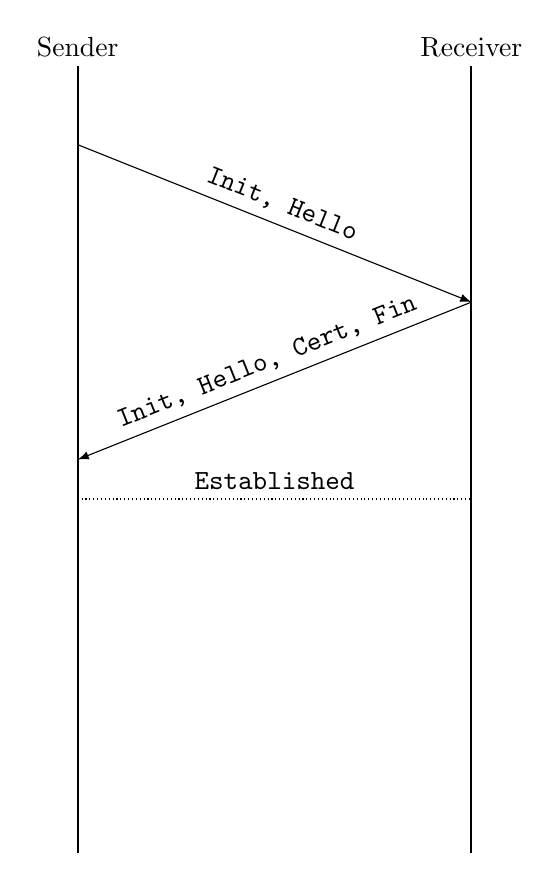
\begin{tikzpicture}[>=latex]
                \coordinate (A) at (2,10);
                \coordinate (B) at (2,0);
                \coordinate (C) at (7,10);
                \coordinate (D) at (7,0);
                \draw[thick] (A)--(B) (C)--(D);
                \draw (A) node[above]{Sender};
                \draw (C) node[above]{Receiver};

                \coordinate (E) at ($(A)!.1!(B)$);
                \draw (E) node[left]{\begin{tabular}{r}
                    \end{tabular}};

                \coordinate (F) at ($(C)!.3!(D)$);
                \draw (F) node[right]{\begin{tabular}{l}
                    \end{tabular}};
                \draw[->] (E) -- (F) node[midway,sloped,above]{\verb$Init, Hello$};

                \coordinate (G) at ($(A)!.5!(B)$);
                \draw (G) node[left]{};
                \draw[->] (F) -- (G) node[midway,sloped,above]{\verb$Init, Hello, Cert, Fin$};

                \coordinate (H) at ($(A)!.55!(B)$);
                \draw (H) node[right]{};

                \coordinate (I) at ($(C)!.55!(D)$);
                \draw (I) node[left]{};
                \draw[densely dotted] (H) -- (I) node[midway,sloped,above]{\verb$Established$};
            \end{tikzpicture}
            \caption{QUIC}
            \label{fig:handshakes:quic}
        \end{subfigure}
        \caption{Handshakes required to establish secure data transmission in the TCP/TLS stack \subref{fig:handshakes:tls} and the QUIC stack \subref{fig:handshakes:quic}. In the case of TCP/TLS we can see that the handshake is substantially more complex and that the TLS handshake requires the full TCP handshake before it can proceed. In both cases these handshakes can be made quicker. In the case of TLS, version 1.3 allows for one less round trip before data can be sent, and in the case of QUIC 0-RTT connection re-establishment may be used in come cases, allowing to send data in the first packet.}
        \label{fig:handshakes_comparison}
    \end{center}
\end{figure}

Compared to TCP/TLS, QUIC combines the transport and cryptographic handshakes in order to minimise the time needed for connection establishment.
A comparison of the handshakes can be seen in Figure \ref{fig:handshakes_comparison}.
TLS is still used to secure QUIC as described by~\citet{thomson_using_2021} unless a different cryptographic protocol is specified.
The initial QUIC handshake keeps the same handshake messages as TLS, however it uses its own framing format, replacing the TLS record layer.
This ensures that the connection is always authenticated and encrypted, unlike in TLS where the initial handshake is still vulnerable.
The combination also means that QUIC typically starts sending data after just one round-trip achieving security by default and lower latency.

\section{The Internet of Things}

It is hard to give a set criterion or definition for which devices qualify as IoT devices.
Generally, an IoT device is a small chip that possesses some processing power and may have embedded sensors.
The key aspect of IoT devices is that they facilitate data exchange with other devices and systems over the Internet.
The modern version of IoT can be attributed to\citepos{weiser_computer_1991} work on ubiquitous computing, although the term itself first appeared in a speech by Peter T. Lewis in 1985.
IoT has applications in various fields, including smart home automation, healthcare, consumer applications, etc.

In terms of classifications within networking and IoT technologies, we can generally split them into wireless and wired, with the former split into short-range, medium-range, and long-range.

Short-range wireless IoT technologies include Bluetooth mesh networks, Z-wave, ZigBee and Wi-Fi, and other lesser-used technologies.
These technologies are the most prevalent in consumer IoT devices, such as smart home applications.
Medium range networks are used heavily in mobile devices with technologies such as LTE and 5G.
The technologies again present an interest due to the amount of traffic that the Internet sees from mobile devices.
On the other hand, long-range networks are rather specific in their applications; for example, VSAT - a satellite communication technology that uses small dish antennas is not something we would necessarily think of when encountering IoT.
Due to the limited application of long-range technologies, we opted to leave them out of our analysis.

Ethernet remains the dominant general-purpose networking standard in terms of wired technologies used by IoT devices.
Although wired technologies provide advantages in terms of data transfer speed, they limit deployments due to the physical wiring constraints.

Having defined what we mean by an IoT device in a network, we now consider the constraints that apply to these devices.
Due to the use cases of IoT, the form factor of these devices should be small.
For example, a processing unit inside a home assistant has to fit in its enclosure.
Additionally, many of these devices have to run for long periods, sometimes on a single lithium battery, hence needing to consume as least energy as possible.
Many use cases of IoT devices also require many of them connected in a mesh network.
For example,~\cite{ericsson_iot_2018} estimated that $0.5$ connected devices were used per square meter in a smart factory, with demand growing.
Large scale deployments add economic constraints to IoT devices as they need to be manufactured from relatively cheap components.

These constraints mean that IoT devices are limited in hardware resources.
Hardware limitations come in three primary forms - CPU power, memory and storage.
Storage in the form of flash memory provides the hardest to solve problems regarding secure data transfer.
The keys required for protocols such as TLS are often large and need to be stored.
For example, the $ESP8266$ controller, a widely used IoT chip, comes with $4$Mb of flash memory.
After installing the firmware and binaries needed, little to no memory may remain for additional storage.

The circumvention of these constraints at the cost of insecure firmware and communication, amongst other issues, is why IoT has become synonymous with security concerns.
Efforts to classify the security issues in the IoT space~\citep{alaba_internet_2017,gupta_security_2021,swamy_security_2017} and create a taxonomy have generally shown several main topics: insecure firmware level code, issues with privacy due to authentication and authorisation and general security concerns due to poor encryption at the transport layer.

Insecure firmware in IoT devices comes from issues with firmware updates and general vulnerabilities stemming from code.
A primary reason is that most programmers opt to create software for IoT devices in memory unsafe languages.
Languages such as C provide the needed efficiency to circumvent processing constraints; however also leave room for memory management issues, leading to vulnerabilities.
When it comes to privacy, a primary goal is ensuring data integrity and confidentiality.
Data sent via the network must not be tampered with nor snooped on by third parties during communication.
Man in the middle attacks is a prime concern for protocols such as MQTT due to their lack of self-imposed encryption.

Hence, finding a way to circumvent the hardware constraints presented by IoT devices and still provide secure data transfer is paramount to the safe adoption of IoT.
Additionally, opting to create IoT firmware code in a memory safe language may prevent vulnerabilities that are present on IoT devices from the moment of deployment.

\section{The Rust programming language}

Rust is a programming language is a modern systems programming language originally created at Mozilla designed to be a highly safe and performant.
It is a systems language that aims to maintain the performance that we expect from languages like C, while also using a unique \textit{ownership} systems in order to maintain memory safety.
Instead of garbage collection Rust opts for a system managed through the resource acquisition is initialisation (RAII) principle~\citep{rust_raii_2021}.
All values have a unique owner and their scope is also tied to this owner.
Hence, by design, Rust does not allow dangling pointers, null pointers and data races as the compiler will not allow for unsafe code to be compiled, without circumventing it using the $unsafe$ keyword.

For example, consider the program written in C in Listing~\ref{lst:C} compared to a similar application in Rust in~\ref{lst:Rust}.
The C program demonstrates a use after free bug.
That is, the pointer is freed and then used in the print statement, resulting in undefined behaviour.
While this example is fairly trivial, in a larger, more complex system these bugs are often very hard to debug and lead to security vulnerabilities.
This issue does not only exist in code bases and organisations with low resources, at the BlueHat security conference, Microsoft researcher~\cite{miller_msrc-security-research2019_02_2019} presented that roughly 70\% of all Microsoft's yearly patches were targeted at fixing memory safety bugs.
On the other hand, the analogous Rust code will not compile due to the ownership system, mitigating this issue all together.

\begin{lstlisting}[language=C, float, caption={An example of a use after free in C code. This is an incorrect use of dynamic memory management, however it compiles. In large, complex code bases, missing bugs such as these often happens and can cause exploitable security issues.}, label=lst:C]
    void bar() {
        int *ptr = (Point *) malloc(sizeof(int));
        free (ptr);
        printf("%d", *ptr); // obvious use after free, however this will compile
    }
\end{lstlisting}

\begin{lstlisting}[language=Rust, float, caption={A similar application in Rust will not compile due to the safety guaranteed by the ownership system. A borrow occurs when $example\_ref$ is assigned to point to $new\_example$, however the ownership system recognises that the borrowed value does not live long enough.}, label=lst:Rust]
    fn bar() {
        let example = String::from("Example");
        let mut example_ref = &example;
        {
            let new_example = String::from("New Example");
            example_ref = &new_example;
        }
        println!("our string is {}", &example_ref); // causes a compiler error in Rust: error `new_example` does not live long enough
    }
\end{lstlisting}

Additionally, due to the focus on concurrency and safe systems programming, Rust has a natural use in networked systems.
However, while Rust aims to be as fast as traditional systems languages, this remains to be seen with even the language's developers saying that the matter of performance is hard to assess~\cite{rust_faq_2021}. Therefore, the interest towards Rust in this project comes from two main aspects.
Firstly, a memory safe language may circumvent the issues with security related bugs in IoT firmware and the supporting network stacks.
As previously discussed, getting the firmware correct on the first try is important in IoT due to the difficulty that comes with updates.
Secondly, assessing the performance of Rust implementations of the QUIC stack is important to solidify Rust as a performant systems programming language.
If the binary sizes produced by the Rust implementations are larger than their C equivalents or if the code is not as performant, then the memory safety guarantees would not matter.
\chapter{Foundational implementations}\label{chap:libs}

This chapter presents the rationale behind our choice of QUIC and MQTT implementations.
In terms of QUIC, we used the $quinn$ implementation in order to create the intermediate library discussed in Chapter~\ref{chapter:quic_socket}.
On the MQTT side, $rumqtt$ was used as the starting point for our MQTT/QUIC implementation.

The choice criteria follow from the previously presented background and some general criteria.
We analysed the available implementations based on their storage footprint, the programming language they were implemented in, their use of TLS, widespread adoption and availability of documentation.

\section{QUIC} \label{section:quic_impl}

In this section, we compare the existing implementations of the QUIC protocol in the context of usability for IoT devices and present the reasoning behind our choice of QUIC library.
We have considered the mainstream implementations in the C, C++, Rust and Go programming languages as these are the languages that can be considered systems languages and would thus be the most widely used ones for IoT devices.
In addition to this, we did not consider implementations paired with a browser web engine as these would be impossible to use on hardware constrained devices.
Hence, we did not include notable implementations such as the QUIC implementation of the chromium web engine~\citep{chromium_quic_2021} and $Neqo$~\citep{mozilla_neqo_2022}.

First, we consider the general landscape of available QUIC implementations to contextualise the ones developed in Rust.
Table~\ref{tab:quics} demonstrates the analysed QUIC implementations.
In order to find the size of the binary, we have used the Linux $ls$ utility.
In the case of the $mvfst$ implementation, we have taken further steps due to the reported binary size being far too large.
Therefore, we had to remove the C++ debug symbols that were causing the binary size to be over 300 MiB.
We have identified the following main methods by which QUIC implementations incorporate TLS:

\begin{itemize}
    \item Use of an external library - the implementation uses an external TLS API either by using a package manager in the case of Rust or by relying on an installed implementation in the case of C and C++.
    \item Use of own implementation - the implementation packages its implementation of the TLS protocol alongside QUIC.
\end{itemize}

This different use of TLS presented a challenge in calculating the binary size of the QUIC servers and clients.

\begin{table}[ht]
    \caption{The identified QUIC implementations and their binary size footprint. The footprint has been split into a client and server footprint using a minimal reproducible example for each. We used each implementation to create an example client and server capable of sending and receiving QUIC packets and analysed the binary size. Where provided, we compared this to the given examples to ensure as little implementation bias as possible. However, this is still not a perfect estimate, and some variance due to implementation details may be present.}\label{tab:quics}
    %\tt 
    \rowcolors{2}{}{gray!3}
    \begin{tabular}{@{}lllll@{}}
        \toprule
        \textbf{Implementation} & \textbf{PL}   & \textbf{Footprint (client) (MiB)} & \textbf{Footprint (server) (MiB)} & \textbf{TLS method} \\
        ngtcp2                  & \texttt{C}    & \texttt{3.4}                      & \texttt{4.3}                      & \texttt{External}   \\
        picoquic                & \texttt{C}    & \texttt{3.2}                      & \texttt{3.9}                      & \texttt{External}   \\
        msquic                  & \texttt{C}    & \texttt{3.2}                      & \texttt{4.1}                      & \texttt{External}   \\
        quic-go                 & \texttt{Go}   & \texttt{8.7}                      & \texttt{9.9}                      & \texttt{External}   \\
        Quinn                   & \texttt{Rust} & \texttt{9.1}                      & \texttt{9.5}                      & \texttt{External}   \\
        Quiche                  & \texttt{Rust} & \texttt{7.8}                      & \texttt{7.0}                      & \texttt{Own}        \\
        mvfst                   & \texttt{C++}  & \texttt{11.1}                     & \texttt{12.0}                     & \texttt{Own}        \\
        \bottomrule
    \end{tabular}
\end{table}

Specifically, in each case, we have considered the external dependencies that a developer will have to install to run the QUIC implementation on a device.
Hence, in the case of C implementations that require an external TLS library, such as OpenSSL, to be installed and linked on the system, we have opted to add the binary size produced by OpenSSL to the size of the QUIC binaries.
Additionally, in the case of $picoquic$, we have added the size of the $picotls$ dependency on top of the size of OpenSSL.

\begin{figure}[ht]
    \centering
    \includegraphics[width=1\linewidth]{images/quic_impls.png}
    \caption{The sizes of the client and server footprints for the selected QUIC implementations. Notable, only Quiche produced a server binary with a smaller size than its corresponding client binary. It is hard to estimate the error margin for the data as this depends on implementation details in the example client and servers.}
    \label{fig:quic_impls}
\end{figure}

Figure~\ref{fig:quic_impls} further visualises the comparison of binary sizes between the various implementations.
This is an important aspect due to the aforementioned hardware constraints.
Notably, we can see that five out of the seven analysed implementations opt to use an external TLS library or engine.
Out of these five, all C implementations supported OpenSSL, with the Go and Rust implementations opting to use a TLS library.
In the case of $quic-go$, this was the $crypto/tls$ package, and in the case of Rust, $rustls$.
We can also see that the Rust implementations are not drastically different in binary footprint size.

In terms of using a memory-safe language, although Go is described as memory safe, it does not opt for compile-time memory safety and instead uses the panic model.
The panic model was the primary reason for the choice of Rust instead of Go, as Rust provides these guarantees using a robust type system.
Between the two Rust implementations - Quinn and Quiche, we chose Quinn due to issues with the Quiche library.
On the other hand, Quiche opts to make the user create a $mio$ event loop, which interfered with the $tokio$ runtime environment used in our chosen MQTT implementation discussed in the next section.
In addition to this, we found that the Quinn API is easier to work with when creating the intermediate library discussed in Chapter~\ref{chapter:quic_socket}; for example, Quinn handles the QUIC handshake in the library and does not require the developer to create an event loop.

\subsection{MQTT}\label{section:mqtt_impls}

Compared to QUIC, the choice of MQTT implementation was substantially simpler.
The criteria for MQTT implementation were that it was developed in Rust, implemented both a client and a broker, had widespread use and adhered to MQTT version 5.0.
Based on the above criteria we identified two possible implementations:\citepos{eclipse_eclipse_2018} $paho$ and $rumqtt$~\citep{bytebeam_rumqtt_2020}.
We opted to use $rumqtt$ at it is a native Rust implementation, whereas $paho$ provides a rust binding to an underlying C implementation.
We chose to evaluate a fully Rust native MQTT/QUIC stack as this provides an opportunity for a valuable comparison to mainstream C implementations.
Other available implementations supported only one side of the MQTT protocol or only supported version 3.1.1.

$Rumqtt$ provides to components for an MQTT application - $rumqttc$ and $rumqttd$.
The former can be used to create an MQTT client, and the latter a broker.
However, the code base for these is somewhat similar, easing the incorporation of QUIC.
Both components provide an interface for supporting asynchronous communication using a $tokio$ runtime, which fits nicely into our choice of QUIC implementation as $Quinn$ requires a $tokio$ environment.
By default, $rumqtt$ uses TCP as its transport layer protocol and TLS through $rustls$.
All underlying implementation assumptions remain equal because this is the same library as $Quinn$ uses.

\section{QuicSocket}\label{chapter:quic_socket}

This section will present $QuicSocket$~\footnote{QuicSocket - \url{https://github.com/Apolexian/QuicSocket}} - the intermediate wrapper API that we developed using $Quinn$ to facilitate establishing a QUIC connection, control streams, and send and receive data.

$QuicSocket$ provides two main types to communicate with $Quinn$ - a $QuicServer$ and a $QuicClient$, and a trait that both of these implement - $QuicSocket$.
The $QuicSocket$ trait defines three function: $new$, $send$ and $recieve$. 
When initialised using the $new$ function, the server and the client attempt to open a QUIC connection.
In the case of the server, it binds to a given port and starts listening for a connection request.
The client binds to a random available port and attempts to connect to a provided URL.
Additionally, in the $new$ function, the server generates a new TLS certificate or reads it from a specified path.
The client's $new$ function must be supplied with the corresponding certificate's path.
If either certificate is not present, the server will reject the connection attempt.
Once a connection has been opened, data transfer can happen.

\begin{lstlisting}[language=Rust, caption={The $send$ function that the $QuicClient$ and $QuicServer$ use for sending data. Data transfer is facilitated by opening a bidirectional stream on the pre-existing connection.}, label=lst:quicsocket_send]
    async fn send(&mut self, payload: Vec<u8>) -> Result<()> {
        let (mut send, _) = self
            .connection
            .open_bi()
            .await
            .map_err(|e| anyhow!("failed to open stream: {}", e))
            .unwrap();
        send.write_all(&payload)
            .await
            .map_err(|e| anyhow!("failed to send request: {}", e))?;
        send.finish()
            .await
            .map_err(|e| anyhow!("failed to shutdown stream: {}", e))?;
        Ok(())
    }
\end{lstlisting}

In order to send data, either side can use the $send$ function demonstrated in Listing~\ref{lst:quicsocket_send}.
We first open a bidirectional stream and then write the provided payload.
Once the client completes writing the payload, it shuts down the stream.
On the other side, the receive function in Listing~\ref{lst:quicsocket_recv} processes the next available QUIC stream and reads the data on it into a supplied buffer.
It then returns the number of bytes written to the buffer.
Hence, to use $QuicSocket$, we must either provide or generate TLS certificates, open a QUIC connection and then use the send and receive functions.
The developed API is analogous to how a TCP socket sends and receives data.
An alternative approach that we considered was to make the $recv$ function return the value that the client or server read from the stream.
However, this approach does not integrate well into any protocol implementation due to the general preference for the buffer pattern.

\begin{lstlisting}[language=Rust, float, caption={The $recv$ function that the $QuicClient$ and $QuicServer$ use for sending data.}, label=lst:quicsocket_recv]
    async fn recv(&mut self, buf: &mut [u8]) -> Result<usize> {
        let (_, mut recv) = self.bi_streams.next().await.unwrap().unwrap();
        let len = recv
            .read(buf)
            .await
            .map_err(|e| anyhow!("failed to read response: {}", e))?;
        Ok(len.unwrap())
    }
\end{lstlisting}

Error handling is handled via the $anyhow$ package throughout the library for idiomatic error handling.
In addition to this, we wrap return values in Rust's $Result$ construct.
Hence, all errors are idiomatically mapped wherever a failure can occur.

An important design choice that we have made when developing $QuicSocket$ is using QUIC streams.
Every call to send and receive in the current implementation creates a bidirectional stream.
An alternate choice was to open a stream at the start of the connection and use it until the connection closes.
However, the latter approach runs into issues when it comes to reading from the stream.
All data was read on one call to receive, which unnaturally coalesced MQTT packets.

Notably, all operations happen asynchronously.
However, as of the implementation time, the Rust standard library does not support asynchronous traits.
The workaround to this issue is using the $async-trait$ crate. 
An unfortunate drawback of using this crate is that every function call results in a heap allocation due to the crate's implementation semantics.
The extra heap allocations do not usually present an issue; however, in the case of hardware constrained devices, this may lead to a bottleneck depending on the usage of the library.
The reasons for not supporting asynchronous traits in Rust are somewhat complex.
For one, an asynchronous function in Rust returns an $impl Future$, meaning that an asynchronous trait would have to support returning $impl Trait$, which it does not.
However, the $async-trait$ crate instead returns a $dyn Future$, the Rust implementation of dynamic dispatch, resulting in a heap allocation but allowing it to be used inside of traits.
We will not further discuss the other reasons for this crate's existence; however,~\cite{matsakis_baby_2019} created a comprehensive analysis of this issue.
Once Rust incorporates asynchronous traits into the language, the heap allocation issue will be resolved, resulting in this problem no longer existing for hardware constrained devices.

In addition to the QUIC specific logic, our goal was also for all communication to happen securely.
Hence, $QuicSocket$ does not accept connection requests without correct TLS keys.
To make working with this easier, we have created functions that handle the creation and reading of TLS keys.

\newpage

\begin{lstlisting}[language=Rust, caption={The $gen_certificates$ function that can be used to generate appropriate TLS certificates.}, label=lst:tls_gen]
    #[allow(unused)]
    #[allow(clippy::field_reassign_with_default)] // https://github.com/rust-lang/rust-clippy/issues/6527
    pub fn gen_certificates() -> Result<(), Box<dyn Error>> {
        let cert = rcgen::generate_simple_self_signed(vec!["localhost".into()]).unwrap();
        let cert_der = cert.serialize_der().unwrap();
        fs::write("./cert.der".to_string(), &cert_der).unwrap();
        let priv_key = cert.serialize_private_key_der();
        fs::write("./key.der".to_string(), &priv_key).unwrap();
        let key = rustls::PrivateKey(priv_key);
        let cert = vec![rustls::Certificate(cert_der.clone())];
        let mut server_crypto = rustls::ServerConfig::builder()
            .with_safe_defaults()
            .with_no_client_auth()
            .with_single_cert(cert, key)?;
        server_crypto.alpn_protocols = ALPN_QUIC_HTTP.iter().map(|&x| x.into()).collect();
        Ok(())
    }
\end{lstlisting}

Listing~\ref{lst:tls_gen} shows the source code of the function that can be used to generate TLS certificates.
The certificates are save to corresponding "key" and "certificate" files and can be distributed to the client and server.
Both the client and server expect certificates to be present when they are run.

\chapter{MQuicTT} \label{chap:port}

This section describes how we used $QuicSocket$ to create a QUIC port of $rumqtt$, the design decisions that we have taken, and possible alternate approaches.

As previously mentioned, $rumqtt$ provides to APIs: $rumqttc$ for creating MQTT clients and $rumqttd$ for creating brokers.
Hence, each of these APIs relies on an underlying TCP implementation to transmit data.
A configuration file is also required for $rumqtdd$ that specifies various parameters such as paths to TLS keys and the ports that MQTT will operate on.
Additionally, $rumqtt$ implements its own layer of TLS to ensure secure communication on top of the TLS layer provided by the underlying transport protocol.

To create $MQuicTT$, we have taken steps that can broadly be summarised in two phases: altering the default TLS code and changing the underlying transport protocol from TCP to QUIC.

As we are working in the domain of hardware constrained devices, providing multiple layers of encryption would be excessive, even for the goal of secure communication.
We can afford for only the transport layer to handle encryption.
Hence, the first step that we have taken is to remove all TLS functionality from both $rumqttd$ and $rumqttc$.

After this, we identified that both APIs have a central interface that controls network communication.
In the case of $rumqttc$ this is the $network$ struct inside $framed.rs$~\footnote{framed.rs - \url{https://github.com/bytebeamio/rumqtt/blob/master/rumqttc/src/framed.rs}} and in the case of $rumqttd$ it is the $network$ struct inside $network.rs$~\footnote{network.rs - \url{https://github.com/bytebeamio/rumqtt/blob/master/rumqttd/src/network.rs}}.
Both of these interfaces use a $tcpstream$ to send and receive data.
The $tcpstream$ is opened when the struct is initialised and closed when the MQTT connection ends.
As TCP is a stateful protocol, minimal connection handling occurs after opening the initial stream.

\begin{lstlisting}[language=Rust, caption={An example of initialising an MQuicTT client. The QUIC connection is established by initialising a $QuicClient$ and the resulting client is passed as an MQTT option.}, label=lst:MQuicTT:client]
    #[tokio::main(worker_threads = 1)]
    async fn main() {
        ...
        let quic_client = QuicClient::new(None).await;
        let mut mqttoptions = MqttOptions::new("test-1", ip, 1883, addr, quic_client);
        mqttoptions.set_connection_timeout(10);
        mqttoptions.set_keep_alive(5);
    
        let (client, mut eventloop) = AsyncClient::new(mqttoptions, 100);
        task::spawn(async move {
            requests(client).await;
        });
    }
\end{lstlisting}

As we have modelled $QuicSocket$ to have an API that closely resembles a typical $tcpstream$ API, the challenge of this stage of the port was managing QUIC streams and the state of connection.
Due to UDP, the protocol underlying QUIC, being stateless, we have handled the connection differently in brokers and clients.

The connection request is sent before an MQTT client object is initialised in the client's case.
Upon successful connection, the programmer must pass the connection to the initialisation function of the client.
This means that a single QUIC connection underpins the client's entire MQTT connection, and streams are used for packets.
Hence, when the client wishes to close the MQTT connection, it also closes the underlying QUIC connection.
In order to do this we have modified the parameters needed to create an $rumqtt$ MQTT client.
An example of the initialisation of a QUIC connection and MQTT client using our implementation is demonstrated in Listing~\ref{lst:MQuicTT:client}.

In the case of a broker, we must wait for a client to send a connection request.
Hence, we may initialise the broker and wait for a QUIC connection, only allowing data transfer when any connection is established.
This also means that the broker does not need to track which connection comes from which client.

\begin{lstlisting}[language=Rust, caption={An example of initialising an MQuicTT broker. We can see that no operations with $QuiSocket$ are required for this initialisation as all QUIC operations are handled internally.}, label=lst:MQuicTT:broker]
    fn main() {
        pretty_env_logger::init();
        let config: Config = confy::load_path("rumqttd.conf").unwrap();
        let mut broker = Broker::new(config);

        let mut tx = broker.link("localclient").unwrap();
        thread::spawn(move || {
            broker.start().unwrap();
        });
        ...
    }

\end{lstlisting}

Hence, as we can see in Listing~\ref{lst:MQuicTT:broker}, the programmer is not required to use any $QuicSocket$ code when creating an $MQuicTT$ broker.

We considered an alternate approach to refactoring the $rumqtt$ codebase to consolidate all network code into a shared internal package.
This would mean that the API for creating a client and broker would be identical and perhaps more ergonomic.
However, we decided not to go with this approach because $rumqttc$ and $rumqttd$ would no longer be disjoint, independent components.
With the chosen approach, it is possible to use different underlying transport protocols for either side, which allows for flexibility in implementation.

Another avenue of discussion stems from $rumqtt$ having two different client implementations: an asynchronous client and an asynchronous client.
In either case, a $tokio$ eventloop is used to handle events.
As $QuicSocket$ requires an asynchronous environment, the natural choice was to use the asynchronous client.
It could however be possible to handle asynchronous events more efficiently by tying the QUIC eventloop to the MQTT eventloop as in the approach described by~\cite{kumar_implementation_2019}.
In our case, we leave the comparison between these two approaches as an avenue for future work.

\chapter{Network simulation}

When evaluating the network performance of the implementations, we considered two options: using real IoT devices or using a network simulation tool.
Due to technical limitations that came with using real devices, such as not being able to access the router of our network, we opted for simulation.
In this chapter, we will discuss how we used Mininet~\citep{lantz_mininet_2021}, a realistic virtual network, in our evaluation.

Mininet is a tool that network developers and researchers can use to create software-defined networks (SNDs) using the $OpenFlow$ standard.

\begin{figure}[ht]
    \centering
    \includegraphics[width=0.5\linewidth]{images/mininet_topo.png}
    \caption{The resulting Dumbbell topology with 5 hosts on either side of the switch. This topology simulates congestion on the link as the hosts have to share it for their data transfer.}
    \label{fig:mininet-topo}
\end{figure}

Using the Python API provided, we created the network topology shown in Figure~\ref{fig:mininet-topo}.
The script takes several parameters to create a simulation environment resembling a realistic scenario.
The variables that the script changes between simulations are the link's \textit{bandwidth}, \textit{delay} and the rate of \textit{packet loss}.

The bandwidth of a link is the maximum rate of data transfer we can achieve.
In contrast to bandwidth in signal processing, we measure bandwidth in bits per second rather than hertz in computer networking.
The delay of a link specifies the latency of the link.
It is the time that a bit of data takes to travel across a link. 
We measure this in milliseconds.
Link delay corresponds to the geographical distance between the communicating parties; however, in the case of IoT, we can expect devices to be in local proximity.
Lastly, the packet loss rate shows the percentage of corrupted or dropped packets in transit.
Various protocols having to retransmit packets also adds to the delay of data transfer.
Importantly, we have only considered the typical circumstances of packet loss and have not included scenarios such as interference or packet loss attacks.

The bandwidth and delay numbers correspond, as closely as possible, to various link types in a network.
To do so, we have gathered data from the~\cite{ofcom_uk_2021} report on UK broadband speeds.
There were specific cases in which it was not possible to find this data in the report; hence it was augmented using a similar methodology in work conducted by~\cite{previdi_is-is_2019} and in the case of ZigBee, the work by~\citet{alena_fault_2011}.

\begin{table}[ht]
    \caption{The parameters chosen for each link simulation in Mininet. The types of links were chosen as the most commonly occurring ones in IoT use cases. The data also assumes a typical IoT setup where most devices are within local geographical proximity. That is, the devices are communicating with each other within the range of one factory or site, with only the central node communicating with some server.}\label{tab:links}
    %\tt 
    \rowcolors{2}{}{gray!3}
    \begin{tabular}{@{}llll@{}}
        \toprule
        \textbf{Simulated Link Type} & \textbf{Link bandwidth (Mb/s)} & \textbf{Link delay (ms)} & \textbf{Packet loss rate (\%)} \\
        Wi-Fi                        & \texttt{30}                    & \texttt{10}              & \texttt{2}                     \\
        ZigBee                       & \texttt{0.25}                  & \texttt{5}               & \texttt{1}                     \\
        4G                           & \texttt{4}                     & \texttt{20}              & \texttt{1.5}                   \\
        3G                           & \texttt{1}                     & \texttt{40}              & \texttt{1.5}                   \\
        100Mb Ethernet               & \texttt{100}                   & \texttt{1}               & \texttt{0.2}                   \\
        \bottomrule
    \end{tabular}
\end{table}

It was complicated to find exact estimates for packet loss rates, with most sources describing approximations for a stable connection~\citep{sdu_ictp-sdu_2013} and not precise measurements.
Hence, the data are best estimates, cross-validated through the different sources and are not exact values.

Using the different links, we then transferred a file of equal size using the various QUIC implementations described in Chapter~\ref{chap:quic_impl} for the evaluation of QUIC implementations.

We evaluated the MQTT/QUIC implementation performance using the same topology and simulation parameters.
In general, MQTT allows for messages with a maximum size of approximately 260MB.
However, this is a huge message, and most publicly deployed brokers will reject it, so a general use-case was simulated.

Each topic in MQTT consists of a hierarchy of topic levels separated by a forward slash.
For example, in a smart home scenario, we may have a topic like $home/groundfloor/kitchen/temp$ to control the temperature in the kitchen via a smart thermostat.
A topic may also include a wildcard.
The topic string $home/groundfloor/+/temp$ includes a \textit{single-level} wildcard that will match an arbitrary string.
This would match the topic $home/groundfloor/lounge/temp$, but not match the topic $home/secondfloor/kitchen/temp$.
If a client wishes to subscribe to multiple topics with the same prefix, a \textit{multi-level} wildcard may be used.
For example, the topic $home/secondfloor/kitchen/\#$ can be used to subscribe to all topics with a prefix matching the string before the hash character.
Notably, brokers reserve topics for system messages starting with the \$ character.

Taking this into account, we opted for a smart home scenario to simulate the MQTT communication.
The data transmitted can be found in Appendix~\ref{appendix:mqtt_message}.
\chapter{Analysis} \label{chapter:eval}

This section presents the analysis results conducted using the previously described methodology.
The analysis is broadly split into two stages: performance analysis and binary size analysis.
The experiment design for the performance analysis can be found in Section~\ref{chap:net_sim}, and the experiment design for the binary analysis can be found in Section~\ref{sec:exp_bin}.
The performance analysis is further split into a connection time analysis and a general transmission time analysis.

\chapter{Network simulation}

When evaluating the network performance of the implementations, we considered two options: using real IoT devices or using a network simulation tool.
Due to technical limitations that came with using real devices, such as not being able to access the router of our network, we opted for simulation.
In this chapter, we will discuss how we used Mininet~\citep{lantz_mininet_2021}, a realistic virtual network, in our evaluation.

Mininet is a tool that network developers and researchers can use to create software-defined networks (SNDs) using the $OpenFlow$ standard.

\begin{figure}[ht]
    \centering
    \includegraphics[width=0.5\linewidth]{images/mininet_topo.png}
    \caption{The resulting Dumbbell topology with 5 hosts on either side of the switch. This topology simulates congestion on the link as the hosts have to share it for their data transfer.}
    \label{fig:mininet-topo}
\end{figure}

Using the Python API provided, we created the network topology shown in Figure~\ref{fig:mininet-topo}.
The script takes several parameters to create a simulation environment resembling a realistic scenario.
The variables that the script changes between simulations are the link's \textit{bandwidth}, \textit{delay} and the rate of \textit{packet loss}.

The bandwidth of a link is the maximum rate of data transfer we can achieve.
In contrast to bandwidth in signal processing, we measure bandwidth in bits per second rather than hertz in computer networking.
The delay of a link specifies the latency of the link.
It is the time that a bit of data takes to travel across a link. 
We measure this in milliseconds.
Link delay corresponds to the geographical distance between the communicating parties; however, in the case of IoT, we can expect devices to be in local proximity.
Lastly, the packet loss rate shows the percentage of corrupted or dropped packets in transit.
Various protocols having to retransmit packets also adds to the delay of data transfer.
Importantly, we have only considered the typical circumstances of packet loss and have not included scenarios such as interference or packet loss attacks.

The bandwidth and delay numbers correspond, as closely as possible, to various link types in a network.
To do so, we have gathered data from the~\cite{ofcom_uk_2021} report on UK broadband speeds.
There were specific cases in which it was not possible to find this data in the report; hence it was augmented using a similar methodology in work conducted by~\cite{previdi_is-is_2019} and in the case of ZigBee, the work by~\citet{alena_fault_2011}.

\begin{table}[ht]
    \caption{The parameters chosen for each link simulation in Mininet. The types of links were chosen as the most commonly occurring ones in IoT use cases. The data also assumes a typical IoT setup where most devices are within local geographical proximity. That is, the devices are communicating with each other within the range of one factory or site, with only the central node communicating with some server.}\label{tab:links}
    %\tt 
    \rowcolors{2}{}{gray!3}
    \begin{tabular}{@{}llll@{}}
        \toprule
        \textbf{Simulated Link Type} & \textbf{Link bandwidth (Mb/s)} & \textbf{Link delay (ms)} & \textbf{Packet loss rate (\%)} \\
        Wi-Fi                        & \texttt{30}                    & \texttt{10}              & \texttt{2}                     \\
        ZigBee                       & \texttt{0.25}                  & \texttt{5}               & \texttt{1}                     \\
        4G                           & \texttt{4}                     & \texttt{20}              & \texttt{1.5}                   \\
        3G                           & \texttt{1}                     & \texttt{40}              & \texttt{1.5}                   \\
        100Mb Ethernet               & \texttt{100}                   & \texttt{1}               & \texttt{0.2}                   \\
        \bottomrule
    \end{tabular}
\end{table}

It was complicated to find exact estimates for packet loss rates, with most sources describing approximations for a stable connection~\citep{sdu_ictp-sdu_2013} and not precise measurements.
Hence, the data are best estimates, cross-validated through the different sources and are not exact values.

Using the different links, we then transferred a file of equal size using the various QUIC implementations described in Chapter~\ref{chap:quic_impl} for the evaluation of QUIC implementations.

We evaluated the MQTT/QUIC implementation performance using the same topology and simulation parameters.
In general, MQTT allows for messages with a maximum size of approximately 260MB.
However, this is a huge message, and most publicly deployed brokers will reject it, so a general use-case was simulated.

Each topic in MQTT consists of a hierarchy of topic levels separated by a forward slash.
For example, in a smart home scenario, we may have a topic like $home/groundfloor/kitchen/temp$ to control the temperature in the kitchen via a smart thermostat.
A topic may also include a wildcard.
The topic string $home/groundfloor/+/temp$ includes a \textit{single-level} wildcard that will match an arbitrary string.
This would match the topic $home/groundfloor/lounge/temp$, but not match the topic $home/secondfloor/kitchen/temp$.
If a client wishes to subscribe to multiple topics with the same prefix, a \textit{multi-level} wildcard may be used.
For example, the topic $home/secondfloor/kitchen/\#$ can be used to subscribe to all topics with a prefix matching the string before the hash character.
Notably, brokers reserve topics for system messages starting with the \$ character.

Taking this into account, we opted for a smart home scenario to simulate the MQTT communication.
The data transmitted can be found in Appendix~\ref{appendix:mqtt_message}.
\section{Connection time comparison} \label{sec:conn_time}
\section{Data transmission comparison}

We next evaluate the time it took both implementations to transmit the aforementioned MQTT messages.
To do so, we have used the previously described methodology.

Based on the analysis of connection time and the previous discussion, we hypothesise that:

\begin{itemize}
    \item \textbf{H1}: $MQuicTT$ performs on-par with $rumqtt$ in the IoT home scenario but does not present a significant difference.
    \item \textbf{H2}: $MQuicTT$ performs significantly better than $rumqtt$ in the printer farm scenario.
    \item \textbf{H3}: $MQuicTT$ can transmit all the messages on all data links in the synthetic scenario, whereas $rumqtt$ is not.
\end{itemize}

Figure~\ref{fig:comm_time} shows the results of this experiment.

\begin{figure}[ht]
    \centering
    \includegraphics[width=1\linewidth]{images/analysis_comm_time.png}
    \caption{The time it took for the implementations to transmit the MQTT messages.
        The base $rumqtt$ implementation is shown in green and $MQuicTT$ in orange.
        Each column represents a scenario, and each row is a data link.
        The time for each Figure is shown in milliseconds. The base implementation of $rumqtt$ could not transmit data in the synthetic packet loss scenario.}
    \label{fig:comm_time}
\end{figure}

We can see that the results support hypothesis \textbf{H1}.
That is,  $MQuicTT$ performs almost identically to $rumqtt$ across all data links for the IoT home scenario.
In fact, $MQuicTT$ actually performs marginally better than $rumqtt$ in this scenario with the transmission time of $MQuicTT$ being on average $2.02\%$ lower than that of $rumqtt$.
From this we can see that $MQuicTT$ presents no disadvantages in terms of transmission time even in network with low packet loss and congestion.

Hypothesis \textbf{H2} however is not supported.
The performance advantage in terms of transmission time for $MQuicTT$ in the printer farm scenario is almost identical to that of the smart home scenario.
On average, $MQuicTT$ transmits the data $2.36\%$ faster than $rumqtt$ and although this is an improvement, it is comparable to the improvement in the IoT home scenario.

The result means that the presented use-case does not present a high enough packet loss percentage for $MQuicTT$ to have a significant advantage.
This can be verified by looking at the synthetic scenario, which validates hypothesis \textbf{H3}.
In the synthetic scenario only $MQuicTT$ managed to transmit the data on all data links and transmitted the data $13.8\%$ faster using ethernet.
Hence, in environments that may experience extreme data loss, $MQuicTT$ presents a clear advantage, however, finding such a scenario may be difficult.

Overall, $MQuicTT$ transmitted the data faster than $rumqtt$ across all scenarios and has shown to be more resilient against high packet loss.
It may however be ineffective overhead to migrate existing deployments to it due to the marginal benefits in low congestion environments.

\section{Binary size experiment design} \label{sec:exp_bin}

The last section of this chapter describes how we have conducted further analysis on the binary size of the QUIC protocol that underlines MQuicTT.
The focus of this section is to see if the QUIC stack contributes a significant overhead to MQuicTT's binary size and how we can reduce this overhead.
We expect that the QUIC stack will contribute to the majority of the size of MQuicTT as MQTT itself is designed to have a low code size overhead.
Hence, the first step of this part of the analysis will be to determine how much QUIC contributes to the binary size.

In order to get a breakdown of the binary we have used the $cargo-bloat$~\footnote{cargo-bloat - \url{https://lib.rs/crates/cargo-bloat}} utility.
The utility analyses the binary using custom ELF, DWARF and Mach-O parsers and disassembles the binary to look for references and links to anonymous data.
Doing so creates a map of the binary that shows where every byte has a label attached to it.

This utility provides the composition of a Rust binary. 
However, it is not perfect and results in some margin of error.
Unfortunately, this margin of error is also not easily measurable.
By comparing the total size of the binary as reported by $cargo-bloat$ to the size reported by the operating system, we have deduced that the total error margin is within $1\%$ with good precision.
This should mean that we can get a somewhat accurate error margin on the components. 
However, it is also possible that the internal calculations are inaccurate despite the overall size being accurate.

The next step in this stage will be analysing methods for trimming down the QUIC stack binary size.
Hence, in this stage, we shift our focus to the binary produced by $QuicSocket$.
To reduce the binary size, we opt to use the method established by~\citet{eggert_towards_2020} as recreating these steps may show a general framework for reducing binary sizes for hardware constrained devices.
Notably, our application already handles client and server code separately; the MQTT broker requires a different binary to the MQTT client.

Hence, the steps we take are as follows:

\begin{itemize}
    \item Compile the binary for a 32-bit target by setting the $target$ flag in cargo to $i686-unknown-linux-gnu$.
    \item Remove any error handling code beyond what is needed for the binary to compile.
    \item Remove any code that writes to standard output.
\end{itemize}

After every step, we record the difference in binary size made by the change using the same methodology.

Once this step is completed we further analyse the size of $Quinn$ and $Rustls$ using a by-function binary size breakdown.
Using the $cargo-bloat$ utility we can get a list of the contribution of each function to the binary size and then assign each function to its respective protocol feature.

\section{Binary size breakdown} \label{sec:binary_sizes}

We first look at an in-depth breakdown of the composition of the binary of the underlying QUIC implementation.
As previously established, hardware constrained devices do not have much space for firmware; hence, identifying sections of the QUIC stack that can be trimmed down or eliminated entirely is essential.
In order to get a breakdown of the binary we have used the $cargo-bloat$~\footnote{cargo-bloat - \url{https://lib.rs/crates/cargo-bloat}} utility.

[figure of results here]

[discussion of results here]

In order to reduce the binary size we opt to use the method established by~\citet{eggert_towards_2020} as recreating these steps may show a general framework for reducing binary sizes for hardware constrained devices.
Notably, our application already handles client and server code separately; the MQTT broker requires a different binary to the MQTT client.

Hence, the steps we have taken are as follows:

\begin{itemize}
    \item Compile the binary for a 32-bit target by setting the $target$ flag in cargo to $i686-unknown-linux-gnu$.
    \item Remove any error handling code beyond what is needed for the binary to compile.
    \item Remove any code that writes to standard output.
\end{itemize}

The resulting binary sizes after these steps can be found in Figure TBA.

[Figure here]

As we can see, after trimming down the binary, the TLS implementation stands out as the most considerable dependency.
While~\cite{eggert_towards_2020} attempts to address this by creating minimal cypher implementations used by TLS, we instead opt to discuss the possibility of a complete alternative to TLS, suitable for hardware constrained devices in Section~\ref{chap:TLS}.


\subsection{Summary}

When discussing the possibility of using a Rust QUIC implementation as the transport layer protocol for network firmware in IoT devices we established that the QUIC implementation must perform at least as well as the baseline and have a binary size which can fit onto widely used IoT devices.

From the above analysis we can conclude that $MQuicTT$ performs at least as well as the baseline TCP implementation of $rumqtt$.
When it comes to connection time, $MQuicTT$ performs marginally better, and when it comes to total transmission time, the implementations are on par.
Hence, this requirement is satisfied.

In terms of binary size we have managed to reduce it to approximately $8Mb$.
This size of binary would easily be installable on popular IoT devices such as the Raspberry Pi 3 Model B, Beagle Board or the Arduino Due.
However, this size of binary would not support industrially-wide used chips such as the esp32.
We have analysed the possible avenues of further reducing the binary size of $MQuicTT$ by addressing issues with the regex library and by analysing $Quinn$ and $Rustls$ by feature.
Hence, overall, we can say that we have achieved creating an implementation that can be used on a large number of IoT devices, but not on ones with stricter hardware constraints.

\chapter{TLS and possible alternatives}\label{chap:TLS}

As we have shown in Section~\ref{sec:binary_sizes}, the TLS implementation size remains the main barrier for secure communication using MQTT.
Hence, in this section, we analyse what exactly TLS provides and possible lightweight alternatives.

[Description of TLS here]

[Description of KP-ABE here]

[Discussion here]
\chapter{Conclusion} \label{chap:conclusion}

We conclude with a brief summary of the work conducted, the developed implementation and results found.
Additionally, we provide a discussion on avenues for future work.

This work has looked at recent developments in the spaces of transport layer protocols and programming languages.
We have aimed to analyse if the technologies, QUIC and Rust, set to succeed current industry standards can be used for IoT network firmware.
The context of IoT provides interesting constraints in terms of the balance of performance, security and hardware constraints.
We have discussed MQTT - the most widely used IoT application layer protocol.
MQTT presents an HTTP like lightweight, publish-subscribe communication system.
We have also shown that MQTT relies on the transport layer to provide transport semantics and secure communication.

By analysing the currently available QUIC and MQTT implementations, we identified libraries that were used as the basis for our implementation.
Both of the selected libraries were developed in the Rust programming language.
Using $Quinn$, we developed an intermediate API - $QuicSocket$ that provides an API for connecting, sending and receiving using QUIC.
Further, we have changed the base $rumqtt$ implementation to use QUIC using this API, resulting in $MQuicTT$ - a QUIC based MQTT implementation.

Using a mininet test bench, we have analysed the performance of the the resulting implementation and have shown that it is comparable to $rumqtt$ in terms of connection time and total transmission time.

We have analysed the binary sizes of the broker and client of $MQuicTT$ and identified the dependencies that contribute the most to the size.
We have shown that Rust's use of $utf-8$ strings can result in size bloat.
Additionally, we have further analysed the contributions made by the QUIC and TLS implementations to devise a methodology for trimming down the QUIC stack.

Overall, we have found that while $MQuicTT$ performed comparably to $rumqtt$, we could not trim down the binary size enough for it to be used on truly hardware constrained devices.
However, the resulting implementation can be used on devices of the Raspberry Pi class.

\section{Future work} \label{sec:future_work}

This section will address the limitations of the work that we have done and discuss future work that would improve or expand upon the topic.
Each section will present a direction for further work and a discussion of it.

\subsection{QUIC implementations}

The number of available QUIC implementations has already far surpassed the number of major TCP implementations that are used in deployments.
Even during the course of this work being produced, a new Rust QUIC implementation was made public - Amazon's $s2n-quic$~\footnote{\url{https://github.com/aws/s2n-quic}}.
The number of QUIC implementations and the difference in direction compared to TCP has several implications on this work.

Firstly, a new more efficient implementation of Rust could be developed that would be a better fit as the base implementation for $MQuicTT$.
Hence, new implementations would need to be analysed.

Secondly, each new implementation means that many servers will have to interface with differing implementations, often with different implementation semantics.
An analysis of how different QUIC implementations perform in conjunction with each other could provide different efficiency statistics to the ones presented in our analysis.
That is, both our broker and clients used $Quinn$ and it would be interesting to analyse if using, for example, $Quinn$ for the broker and $s2n-quic$ for the client, impacts performance.

Additionally, with so many implementations having to interface with each other, it would be worthwhile to analyse the number of bugs in QUIC deployments compared to TCP ones.

\subsection{Binary analysis}

As discussed, all binary analysis for this work was conducted manually.
This task is rather tedious and error prone.
While it is possible to create a dependency analyser and a decompiler to analyse the binaries, it is currently impossible to connect this automatically with different features of a protocol.

For this to be possible we would need to augment protocol implementations with some sort of indication of a feature.
In the Rust programming language this could be done via a macro.
For example, a function with the macro $\#[feature(VersionNegotation)]$ could be used to indicate Quic's version negotiation feature.
This method, however, can be viewed as quite restrictive as it essentially enforces a by-feature abstraction.
As we have seen in $Quinn$, this is not always the way developers want to write their code.

Hence, to be able to conduct this sort of analysis we would need to find an nonintrusive way of augmenting implementations with such details.

\subsection{Comparison analysis to CoAP}

We have previously discussed the similarities between using QUIC for MQTT and using CoAP.
Both methods utilise UDP and an HTTP style messaging approach.
Additionally, both provide retalitevly low code overhead, which is important for hardware constrained devices.

While this work did not focus on the comparison of $MQuicTT$ to CoAP, such an analysis would be crucial to understanding the performance of QUIC in IoT.
An additional avenue of future work is extracting the core features that both these approaches share and analysing if they could be employed to make other protocols better for hardware constrained devices.
The result of such work could create a general approach to creating protocols for IoT devices.

\subsection{Improved test bench}

There are several avenues that could be taken for improving the analysis test bench that we used.
Firstly, a remote controller could be implemented for the mininet topology to be able to use an actual mesh topology, with cycles, instead of the minimum spanning tree one deployed for this work.
This would also mean that different load balancing and routing options could be tested for the scenarios, to better replicate a realistic deployment.
This would also mean that network failures, such as switches going offline, could be simulated programmatically.
Naturally, a hardware test bench analysis would also improve any further work.
\begin{appendices}
    \input{chapters/appendecies/data.tex}
    \chapter{MQTT simulation messages}\label{appendix:mqtt_message}
    \chapter{Mininet Topology Definition}\label{appendix:topo}

The full mininet topology definition via the $dump$ and $links$ command. The Python API definition can also be found on GitHub~\footnote{Topology - \url{https://github.com/Apolexian/level4-scripts/blob/master/mesh_topo/mesh.py}}.

\begin{lstlisting}[caption={Mininet $links$ on the used topology.}, label=lst:app:topo]

    Links:
    
    h00-eth1<->h01-eth1 (OK OK) h00-eth2<->h02-eth1 (OK OK) 
    h00-eth3<->h03-eth1 (OK OK) h00-eth4<->h04-eth1 (OK OK) 
    h01-eth2<->h02-eth2 (OK OK) h01-eth3<->h03-eth2 (OK OK) 
    h01-eth4<->h04-eth2 (OK OK) h02-eth3<->h03-eth3 (OK OK) 
    h02-eth4<->h04-eth3 (OK OK) h03-eth4<->h04-eth4 (OK OK) 
    h10-eth1<->h11-eth1 (OK OK) h10-eth2<->h12-eth1 (OK OK) 
    h10-eth3<->h13-eth1 (OK OK) h10-eth4<->h14-eth1 (OK OK) 
    h11-eth2<->h12-eth2 (OK OK) h11-eth3<->h13-eth2 (OK OK) 
    h11-eth4<->h14-eth2 (OK OK) h12-eth3<->h13-eth3 (OK OK) 
    h12-eth4<->h14-eth3 (OK OK) h13-eth4<->h14-eth4 (OK OK) 
    s0-eth1<->h00-eth0 (OK OK) s0-eth2<->h01-eth0 (OK OK) 
    s0-eth3<->h02-eth0 (OK OK) s0-eth4<->h03-eth0 (OK OK) 
    s0-eth5<->h04-eth0 (OK OK) s0-eth6<->s9-eth2 (OK OK) 
    s1-eth1<->h10-eth0 (OK OK) s1-eth2<->h11-eth0 (OK OK) 
    s1-eth3<->h12-eth0 (OK OK) s1-eth4<->h13-eth0 (OK OK) 
    s1-eth5<->h14-eth0 (OK OK) s1-eth6<->s9-eth3 (OK OK) 
    s9-eth1<->h9-eth0 (OK OK)
        
    \end{lstlisting}

\begin{lstlisting}[caption={Mininet $dump$ on the used topology.}, label=lst:app:topo]

Dump:

<Host h00: h00-eth0:10.0.0.1,h00-eth1:None,h00-eth2:None,h00-eth3:None,h00-eth4:None pid=17658> 
<Host h01: h01-eth0:10.0.0.2,h01-eth1:None,h01-eth2:None,h01-eth3:None,h01-eth4:None pid=17660> 
<Host h02: h02-eth0:10.0.0.3,h02-eth1:None,h02-eth2:None,h02-eth3:None,h02-eth4:None pid=17662> 
<Host h03: h03-eth0:10.0.0.4,h03-eth1:None,h03-eth2:None,h03-eth3:None,h03-eth4:None pid=17664> 
<Host h04: h04-eth0:10.0.0.5,h04-eth1:None,h04-eth2:None,h04-eth3:None,h04-eth4:None pid=17666> 
<Host h9: h9-eth0:10.0.0.6 pid=17668> 
<Host h10: h10-eth0:10.0.0.7,h10-eth1:None,h10-eth2:None,h10-eth3:None,h10-eth4:None pid=17670> 
<Host h11: h11-eth0:10.0.0.8,h11-eth1:None,h11-eth2:None,h11-eth3:None,h11-eth4:None pid=17672> 
<Host h12: h12-eth0:10.0.0.9,h12-eth1:None,h12-eth2:None,h12-eth3:None,h12-eth4:None pid=17674> 
<Host h13: h13-eth0:10.0.0.10,h13-eth1:None,h13-eth2:None,h13-eth3:None,h13-eth4:None pid=17676> 
<Host h14: h14-eth0:10.0.0.11,h14-eth1:None,h14-eth2:None,h14-eth3:None,h14-eth4:None pid=17678> 
<OVSSwitch s0: lo:127.0.0.1,s0-eth1:None,s0-eth2:None,s0-eth3:None,s0-eth4:None,s0-eth5:None,
    s0-eth6:None pid=17683> 
<OVSSwitch s1: lo:127.0.0.1,s1-eth1:None,s1-eth2:None,s1-eth3:None,s1-eth4:None,s1-eth5:None,
    s1-eth6:None pid=17686> 
<OVSSwitch s9: lo:127.0.0.1,s9-eth1:None,s9-eth2:None,s9-eth3:None pid=17689> 
<Controller c0: 127.0.0.1:6653 pid=17651> 

\end{lstlisting}


\end{appendices}
\bibliographystyle{abbrvnat}
\bibliography{l4proj}
\end{document}
